
\documentclass[11pt,a4paper]{article}
\usepackage[utf8]{inputenc}
\usepackage{amsmath, amssymb, amsthm}
\usepackage{geometry}
\usepackage{graphicx} % Include graphics
\usepackage{hyperref} % Hyperlinks
\usepackage{enumerate} % Customizable enumeration
\geometry{a4paper, margin=1in}

\theoremstyle{plain}
\newtheorem{theorem}{Theorem}[section]
\newtheorem{lemma}[theorem]{Lemma}
\newtheorem{proposition}[theorem]{Proposition}
\newtheorem{corollary}[theorem]{Corollary}
\theoremstyle{definition}
\newtheorem{definition}[theorem]{Definition}
\newtheorem{example}[theorem]{Example}
\newtheorem*{definition*}{Definition}
\theoremstyle{remark}
\newtheorem*{remark}{Remark}
\newtheorem*{note}{Note}

\begin{document}

% \tableofcontents

\setcounter{section}{2} 
\section{Chapter 3 - Finding the bounds}

\subsection{Discretising Theorem 1}

We attempt to now discretise Theorem 1. To do this, we refer to the original proof, and note the points at which the proof relies on the continuity of the function space. We then attempt to replace these points with discrete analogs, and verify if an analogous result holds in this new discrete space.

We are required to find an analogous result for Proposition 2.1 - one where we assume that we can only observe finitely many samples of \(f\) on a uniform mesh.

\[
    \|f - P_{m}(f)\|_{p,[-\pi,\pi]^s} \leq \frac{c}{m^r} \|f\|_{W^{p*}_{r,s}} 
\]

The aim being to find some bound for \(f\) in the discrete space instead. The idea behind the original proof of Theorem 1, was that given the fact that we have this polynomial approximation for functions in the continuous sobolev space, we can use this to find a bound for the error between the function and the neural network approximation, by further approximating the polynomial approximation by derivatives of \(\phi \) our activation function.

We aim to add a further layer to this by considering the error between the discrete and continuous spaces. Hoping to then substitute this in the inequality above, and find a bound for the error between some \(f_{\text{discrete} }\) in our discrete space and the shallow network approximation of \(f\).

\begin{proposition}[Error between Discrete and Continuous Spaces]
We begin by considering the error between discrete and continuous Sobolev norms. For a function \( u_h \) defined on a discrete set of nodes on a uniform mesh \( \Omega_h \subset \Omega \subset \mathbb{R}^n \) with spacing \( h \), and a function \( u \) defined on a continuous domain \( \Omega \), the error between the discrete and continuous norms can be estimated by:

\begin{align*}
    \text{Error} &= \left\| \|u_h\|_{h,k,p} - \|u\|_{W^{k,p}(\Omega)} \right\|_{L^p}\\
     &= \left\| \left( \sum_{|\alpha| \leq k} \|D^\alpha_h u_h\|_{l^p_h(\Omega_h)}^p \right)^{1/p} - \left( \sum_{|\alpha| \leq k} \|D^\alpha u\|_{L^p(\Omega)}^p \right)^{1/p} \right\|_{L^p}
\end{align*}

where \( D^\alpha_h \) represents the discrete derivatives calculated using finite differences, and \( D^\alpha \) represents the weak derivatives of \( u \).

This error encapsulates the differences due to the discretization of derivatives and the integration (or summation) over the domain.

% We have that for

% \[
% \text{Error}_\alpha = \left| \|D^\alpha_h u_h\|_{l^p_h(\Omega_h)} - \|D^\alpha u\|_{L^p(\Omega)} \right|
% \]

% \[
%     \text{Error} \leq  \left( \sum_{|\alpha| \leq k} \text{Error}_{\alpha}^{p} \right)^{1/p}
% \]


% We compute \( \text{Error}_{\alpha} \) explicitly.
The error \( E \) in approximating \( D^\alpha u \) by \( D_h^\alpha u_h \) at a point \( \mathbf{x} \) is:
\[
E = D^\alpha u(\mathbf{x}) - D_h^\alpha u_h(\mathbf{x})
\]

Using Taylor's theorem, the function \( u \) around \( \mathbf{x} \) can be expanded as:
\[
u(\mathbf{x} + h\mathbf{e}_i) \approx u(\mathbf{x}) + hu_i'(\mathbf{x}) + \frac{h^2}{2}u_i''(\mathbf{x}) + \cdots
\]
for small \( h \), where \( u_i' \), \( u_i'' \), etc., denote derivatives of \( u \) at \( \mathbf{x} \).

Generalizing this to a multi-index derivative using forward differences:
\[
u(\mathbf{x} + h\alpha) = u(\mathbf{x}) + h |\alpha| Du(\mathbf{x}) + \frac{h^2}{2} D^2u(\mathbf{x}) \cdot \alpha + \cdots
\]

Substituting in the approximation for \( u_h(\mathbf{x} + h\alpha) \):
\[
D_h^\alpha u_h(\mathbf{x}) = \frac{u(\mathbf{x} + h\alpha) - u(\mathbf{x})}{h^{|\alpha|}} \approx \frac{1}{h^{|\alpha|}} \left(h |\alpha| Du(\mathbf{x}) + \frac{h^2}{2} \sum_{i=1}^n \alpha_i u_{ii}''(\mathbf{x}) + O(h^3)\right)
\]
\[
D_h^\alpha u_h(\mathbf{x}) \approx D^\alpha u(\mathbf{x}) + h \sum_{i=1}^n \alpha_i u_{ii}''(\mathbf{x}) + O(h^2)
\]

Thus, the error \( E \) can be approximated as:
\[
E \approx h \sum_{i=1}^n \alpha_i u_{ii}''(\mathbf{x}) + O(h^2)
\]

Given that \( E \) approximates the pointwise error for the derivative approximations, for the \( L^p \) norm of this error across a domain \( \Omega \), we can estimate:
\[
\| E \|_{L^p(\Omega)} \approx \| h \sum_{i=1}^n \alpha_i u_{ii}'' \|_{L^p(\Omega)} + O(h^2)
\]
Here, the norm \( \| \cdot \|_{L^p(\Omega)} \) denotes the \( L^p \) norm over the domain \( \Omega \), applying to each derivative error estimate separately.

\paragraph*{Aggregate Error Across All Derivatives}

When summing over all \( \alpha \) where \( |\alpha| \leq k \), the total error in terms of the \( L^p \) norms of all derivatives up to order \( k \) would be:
\[
\left\| \left(\sum_{|\alpha| \leq k} \| D^\alpha u_h - D^\alpha u \|_{L^p(\Omega_h)}^p \right)^{1/p} \right\| \approx \left\| \left( \sum_{|\alpha| \leq k} \left(h \sum_{i=1}^n \alpha_i \| u_{ii}'' \|_{L^p(\Omega)} \right)^p \right)^{1/p} \right\| + O(h^2)
\]
This formula indicates that the aggregate error is a function of \( h \), scaled by the \( L^p \) norms of the second derivatives of \( u \), summed appropriately over all relevant multi-indices and directions.

\paragraph*{Inequality Formulation}

We can thus express the error inequality for the \( L^p \) norm of the derivative norms as:
\[
\text{Error} = \| u_h \|_{h,k,p} - \| u \|_{W^{k,p}(\Omega)} \leq C h \sum_{|\alpha| \leq k} \sum_{i=1}^n \alpha_i \| u_{ii}'' \|_{L^p(\Omega)} + O(h^2)
\]
where \( C \) is a constant that may depend on \( k \), \( n \), and \( p \).



This inequality provides a theoretical upper bound on the error between the numerical approximation \( u_h \) and the true function \( u \) in the Sobolev space defined by \( W^{k,p} \) norms, indicating how the error behaves as a function of the mesh size \( h \) and the smoothness of \( u \).
\end{proposition}

\begin{proposition}

We now combine the necessary inequalities.

\begin{enumerate}
    \item \textbf{First Inequality:}
    \[
    \|f - f_{\text{discrete}}\| \leq Ch \sum_{|\alpha| \leq k} \sum_{i=1}^n \alpha_i \|f_i''\|_{L^p(\Omega)} + O(h^2)
    \]
    This suggests the norm of the error between a function \(f\) and its discrete approximation \(f_{\text{discrete}}\) is bounded by a term linearly dependent on \(h\) and the \(L^p\) norms of second derivatives of \(f\), plus higher order terms.
    
    \item \textbf{Second Inequality:}
    \[
    \|f - P_m(f)\|_{L^p([-\pi , \pi]^s)} \leq \frac{C}{m^r} \|f\|_{W^{p^*}_{r,s}}
    \]
    This represents the error bound when approximating \(f\) by a projection \(P_m(f)\) using some polynomial basis functions, with the error decaying as \(m^r\).
\end{enumerate}

\paragraph*{Goal:}

We need to find an expression for:
\[
\|f_{\text{discrete}} - P_m(f)\|
\]

\paragraph*{Approach:}

We will use the triangle inequality to link the given expressions:
\[
\|f_{\text{discrete}} - P_m(f)\| \leq \|f_{\text{discrete}} - f\| + \|f - P_m(f)\|
\]

Plugging in the bounds provided by the first two inequalities, we get:
\[
\|f_{\text{discrete}} - P_m(f)\| \leq (Ch \sum_{|\alpha| \leq k} \sum_{i=1}^n \alpha_i \|f_i''\|_{L^p(\Omega)} + O(h^2)) + \left(\frac{C}{m^r} \|f\|_{W^{p^*}_{r,s}}\right)
\]

\paragraph*{Simplifying:}

Since both terms provide bounds rather than exact values, and assuming that constants may differ when summing these bounds, the inequality becomes:
\[
\|f_{\text{discrete}} - P_m(f)\| \leq C'\left(h \sum_{|\alpha| \leq k} \sum_{i=1}^n \alpha_i \|f_i''\|_{L^p(\Omega)} + \frac{1}{m^r} \|f\|_{W^{p^*}_{r,s}} + O(h^2)\right)
\]

Here \(C'\) is a new constant that encapsulates any constant factors from both terms, and \(O(h^2)\) represents higher-order small terms in \(h\).

This inequality indicates that the approximation error between the discrete version of \(f\) and its polynomial projection is controlled both by the discretization step size \(h\) and the number of terms \(m\) in the polynomial projection, as well as the smoothness of \(f\). This is useful for analyzing numerical schemes where both spatial discretization and modal truncation errors contribute to the overall approximation error.

Note however, that the above inequality is a relationship between our polynomial approximation of our underlying function \(f\) in the continuous space and samples of this function on a uniform mesh \(f_{\text{discrete} }\). 

Use of this inequality is not relevant for the case where we are attempting to approximate just the ground-truth reality of \(f_{\text{discrete} }\) by a shallow network - for that we would have to find another equivalent proposition on how to approximate \(f_{\text{discrete} }\) with a polynomial basis itself, and join the inequalities in a similar fashion. Here we are hoping to still approximate the underlying continuous function \(f\).

\[
    \| P_m(f) - N_n(f) \|_{\infty} \leq cm^{-r} \| f \|_{W_r^p, s}.
\]

\[
    \|f_{\text{discrete}} - P_m(f)\| \leq C'\left(h \sum_{|\alpha| \leq k} \sum_{i=1}^n \alpha_i \|f_i''\|_{L^p(\Omega)} + \frac{1}{m^r} \|f\|_{W^{p^*}_{r,s}} + O(h^2)\right)
\]

\[
    \| f_{\text{discrete} } - N_{n}(f) \| \leq \ ?
\]

\end{proposition}

\begin{theorem}[Discretised Theorem 1]

    For a target function \(f \in W^{p}_{r,s}\) the continuous Sobolev space, we take \(f_{\text{discrete} } \) the function \(f\) sampled at a uniform mesh over its domain. We have that for a shallow network \(N_n\) with \(n\) neurons in its hidden layer, the error between the function \(f_{\text{discrete} }\) and its shallow network approximation \(N_n(f)\) can be bounded by:
    \[
   \|f_{\text{discrete}} - N_n(f)\| \leq C'' \left( h \sum_{|\alpha| \leq k} \sum_{i=1}^n \alpha_i \|f_i''\|_{L^p(\Omega)} + n^{-r/s} \|f\|_{W^{p^*,s}_r} + O(h^2) \right)
    \]

    Equivalently;
    We define \( E(h, n, f) \) as an error term that includes contributions from discretization error and higher-order terms in \( h \). This error term can be expressed as:
    \[
    E(h, n, f) = h \sum_{|\alpha| \leq k} \sum_{i=1}^n \alpha_i \|f_i''\|_{L^p(\Omega)} + O(h^2)
    \]

    Now, substituting this back into the inequality, we can write:
    \[
    \|f_{\text{discrete}} - N_n(f)\| \leq C'' \left( n^{-r/s} \|f\|_{W^{p^*,s}_r} + E(h, n, f) \right)
    \]
    
\end{theorem}

% \begin{proof}
% \begin{enumerate}
%     \item Approximation Error Between \( P_m(f) \) and \( N_n(f) \):
%     \[
%     \| P_m(f) - N_n(f) \|_\infty \leq cm^{-r} \| f \|_{W^{p^*}_{r,s}}
%     \]
%     This inequality suggests that the error between the polynomial projection \( P_m(f) \) and another numerical approximation \( N_n(f) \) decreases with \( m^r \), where \( r \) is related to the order of the projection or numerical method and \( m \) is the number of terms in the approximation.

%     \item Approximation Error Between \( f \) and \( P_m(f) \) by \( f_{\text{discrete}} \):
%     \[
%     \| f_{\text{discrete}} - P_m(f) \| \leq C' \left( h \sum_{|\alpha| \leq k} \sum_{i=1}^n \alpha_i \| f_i'' \|_{L^p(\Omega)} + \frac{1}{m^r} \| f \|_{W^{p^*}_{r,s}} + O(h^2) \right)
%     \]
%     Here, the error is controlled by the discretization step \( h \), the order of derivatives \( k \), and the polynomial approximation order \( m \).
% \end{enumerate}

% \paragraph*{Goal:} Estimate \( \| f_{\text{discrete}} - N_n(f) \| \)

% Using the triangle inequality, we can combine these two to find the error between \( f_{\text{discrete}} \) and \( N_n(f) \):
% \[
% \| f_{\text{discrete}} - N_n(f) \| \leq \| f_{\text{discrete}} - P_m(f) \| + \| P_m(f) - N_n(f) \|
% \]

% Substitute the bounds from the given inequalities:
% \[
% \| f_{\text{discrete}} - N_n(f) \| \leq C' \left( h \sum_{|\alpha| \leq k} \sum_{i=1}^n \alpha_i \| f_i'' \|_{L^p(\Omega)} + \frac{1}{m^r} \| f \|_{W^{p^*}_{r,s}} + O(h^2) \right) + cm^{-r} \| f \|_{W^{p^*}_{r,s}}
% \]

% Simplifying; the terms \( \frac{1}{m^r} \| f \|_{W^{p^*}_{r,s}} \) are present in both components, suggesting a potential for simplification. We can factor out common terms and aggregate constants:
% \[
% \| f_{\text{discrete}} - N_n(f) \| \leq C'' \left( h \sum_{|\alpha| \leq k} \sum_{i=1}^n \alpha_i \| f_i'' \|_{L^p(\Omega)} + \frac{1}{m^r} \| f \|_{W^{p^*}_{r,s}} + O(h^2) \right)
% \]
% where \( C'' \) represents an aggregate constant, potentially larger than \( C' \) and \( c \), reflecting the combined effects of discretization and numerical approximation.

% This derived inequality provides an upper bound on the error between the discrete approximation of \( f \) and another numerical approximation \( N_n(f) \), incorporating the influence of mesh size \( h \), the smoothness and derivatives of \( f \), and the number of terms \( m \) in the polynomial projection.
% \end{proof}

%%%%%%%%%%%%%%%%%%%%%%%%%%%%%%%%%%%%%%%%%%%%%%%%%%%%%%%%%%%%%%%%%%%%%%%%%%%%%%

\begin{proof}
    We begin by considering the previous inequalities
\begin{enumerate}
    \item \textbf{Error between \( P_m(f) \) and \( N_n(f) \)} (Infinity Norm):
    \[
    \|P_m(f) - N_n(f)\|_{\infty} \leq cm^{-r} \|f\|_{W^{p^*,s}_r}
    \]
    This inequality is already provided in the \( L^\infty \) norm. From the proof of Theorem 1.

    \item \textbf{Error between \( f_{\text{discrete}} \) and \( P_m(f) \)}:
    \[
    \|f_{\text{discrete}} - P_m(f)\| \leq C' \left( h \sum_{|\alpha| \leq k} \sum_{i=1}^n \alpha_i \|f_i''\|_{L^p(\Omega)} + \frac{1}{m^r} \|f\|_{W^{p^*,s}_r} + O(h^2) \right)
    \]
\end{enumerate}

\paragraph*{Applying Norm Relationship}

Using the norm relationship \( |g|_{L^p} \leq 2^{s/p} |g|_{\infty} \) to the difference \( P_m(f) - N_n(f) \), we can express the \( L^p \) norm:
\[
\|P_m(f) - N_n(f)\|_{L^p} \leq 2^{s/p} \|P_m(f) - N_n(f)\|_{\infty} \leq 2^{s/p} cm^{-r} \|f\|_{W^{p^*,s}_r}
\]

\paragraph*{Using the Triangle Inequality}

Combining errors through the triangle inequality:
\[
\|f_{\text{discrete}} - N_n(f)\| \leq \|f_{\text{discrete}} - P_m(f)\| + \|P_m(f) - N_n(f)\|_{L^p}
\]

Substitute the bounds:
\[
\|f_{\text{discrete}} - N_n(f)\| \leq C' \left( h \sum_{|\alpha| \leq k} \sum_{i=1}^n \alpha_i \|f_i''\|_{L^p(\Omega)} + \frac{1}{m^r} \|f\|_{W^{p^*,s}_r} + O(h^2) \right) + 2^{s/p} cm^{-r} \|f\|_{W^{p^*,s}_r}
\]

\paragraph*{Simplifying}

Assuming that \( m \) scales with \( n \) such that \( m \sim n^{1/s} \)
\[
\|f_{\text{discrete}} - N_n(f)\| \leq C'' \left( h \sum_{|\alpha| \leq k} \sum_{i=1}^n \alpha_i \|f_i''\|_{L^p(\Omega)} + n^{-r/s} \|f\|_{W^{p^*,s}_r} + O(h^2) \right)
\]
where \( C'' \) might now encapsulate \( 2^{s/p} c \) and other constants.

This formulation provides a comprehensive upper bound that reflects both discretization and numerical approximation errors, explicitly incorporating the decay rate \( n^{-r/s} \) as influenced by the polynomial degree and the structure of the Sobolev space.
\end{proof}

\subsection{Empirical Tests}

We now aim to empirically test the bounds provided by Theorem 1, and its discretisation and Proposition 2.1. We will consider a simple function \( f \) and its discrete version \( f_{\text{discrete}} \), and approximate these using a shallow network \( N_n \) with varying numbers of neurons in its hidden layer. We will then compare the approximation errors to the bounds derived in the previous sections.

\subsubsection{Impact of Grid Resolution}

We first explore the case for a simple function \( f \) defined on a 1D domain \( \Omega = [-1, 1] \). We sample this function at a uniform mesh with varying resolutions \( h \), generating the discrete function \( f_{\text{discrete}} \). We then approximate this function using a shallow network \( N_n \) with varying numbers of neurons in its hidden layer. The goal is to observe how the approximation error changes with grid resolution and network complexity.

We ran 25 trials, each training a shallow network for 50 epochs with varying widths \( n = 1 \to 2500 \). We did this 3 times for mesh resolutions \( h = 10, 100, 1000 \). The average final losses (with respect to the \(L^2\) norm) across trials for each resolution are shown below.


\begin{figure}[h]
    \centering
    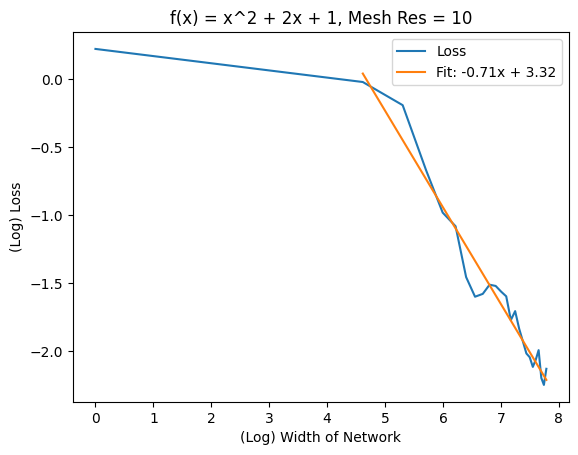
\includegraphics[width=0.8\textwidth]{figures/h-10.png}
    \caption{}
    \label{fig:}
\end{figure}
\begin{figure}[h]
    \centering
    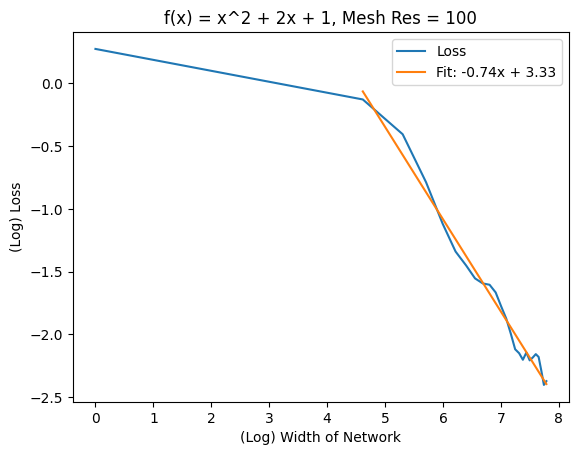
\includegraphics[width=0.8\textwidth]{figures/h-100.png}
    \caption{}
    \label{fig:}
\end{figure}
\begin{figure}[h]
    \centering
    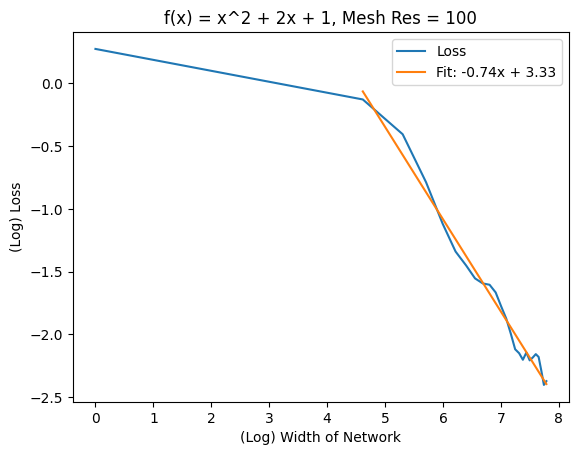
\includegraphics[width=0.8\textwidth]{figures/h-100.png}
    \caption{}
    \label{fig:}
\end{figure}

\subsubsection{Examples of Various Gradients}

We now take the following set of examples to see if the bounds hold true for a variety of functions. We consider the following functions:

\begin{enumerate}
    \item \( f(x) = x^{2} + 2x + 1 \)
    \item \( f(x) = \sin(x) \)
    \item \( f(x) = \sqrt{x+1} \)
    \item \(f(x) = \exp(-x^{2} )\) 
    \item \(f(x) = \left\vert x \right\vert \) 
    \item \(f(x,y ) = \left\lVert x^{2} -y^{2} \right\rVert \)
    \item \(f(x,y,z) = \left\lVert x^{2} - y^{2} + z^{2} \right\rVert \)
\end{enumerate}

% Create table of functions, expected gradients, and observed gradients

\begin{table}[h]
    \centering
    \begin{tabular}{c|c|c|c}
        \toprule
            \(f\)  & Sobolev Space & Expected Gradient & Observed Gradient  \\
        \midrule
            \(x^{2}  + 2x + 1\)  &   & \(-\frac{1}{2}\)   &   \\
            \(\sin (x)\)  &   & \(-1\) &   \\
            \(\sqrt{x+1} \)  &   & \(-\frac{1}{2}\)   &   \\
            \(\exp (-x^{2})\)  &   & \(-2\)  &   \\
            \(\left\vert x \right\vert \)  &   & \(-1\)  &   \\
            \(\left\lVert x^{2} -y^{2} \right\rVert \)  &   & \(-\frac{1}{2}\)  &   \\
        \bottomrule
    \end{tabular}
    \caption{Functions to test Theorem 1}
    \label{tab:label}
\end{table}

% 
\begin{table}[h]
    \centering
    \begin{tabular}{|c|c|c|c|}
    \hline
    \textbf{f} & \textbf{Sobolev Space} & \textbf{Expected Gradient} & \textbf{Observed Gradient} \\
    \hline
    \(x^2 + 2x + 1\) & \(W^{2}_{\infty,1}\) & \(-\frac{1}{2}\) &  \\
    \(\sin(x)\) & \(W^{2}_{\infty,1}\) & \(-1\) &  \\
    \(\sqrt{x+1}\) & \(W^{2}_{1,1}\) & \(-\frac{1}{2}\) &  \\
    \(\exp(-x^2)\) & \(W^{2}_{\infty,1}\) & \(-2\) &  \\
    \(|x|\) & \(W^{2}_{1,1}\) & \(-1\) &  \\
    \(\|x^2 - y^2\|\) & \(W^{2}_{1,2}\) & \(-\frac{1}{2}\) &  \\
    \hline
    \end{tabular}
    \label{tab:label}
\end{table}
% 


For each we ran the test for 1000 samples on the domain \([-1,1]^s\)  and 50 epochs for 25 trials, and shallow network widths of \(n = 1 \to 2500\). The average final losses for each function are shown below. For each of the tests we fixed the mesh resolution at \(h = 100\), as a result of computational constraints, higher resolutions were prohibitively expensive.
We take the log-log-plot of each - and see if we can observe the expected gradient of \(-\frac{r}{s}\) for large \(n\), where \(r\) is the order of the Sobolev space( the differentiablity of our target function) and \(s\) the dimension of the domain of our target function.


\end{document}